\newpage
\section{Uitvoerbaarheid Strategie\"{e}n}
\label{h6}

\subsection*{Deelvraag 3: Welke strategie is per specifieke bevolkingsgroep aan te bevelen wanneer zij de regel van van voorkeursdrempel in de kieswet in hun voordeel willen benutten?}
Zoals in het vorige hoofdstuk al is beschreven kunnen de vier verschillende bevolkingsgroepen uit meerdere strategie\"{e}n kiezen die een hoog rendement kunnen leveren. Daarmee lijkt de derde deelvraag makkelijk te beantwoorden. De bevolkingsgroepen kunnen simpelweg de strategie kiezen waarvan berekend is dat deze het hoogste rendement heeft. Of een strategie de voorkeur geniet boven een andere strategie ligt niet enkel aan het aantal zetels dat een strategie kan opleveren. De keuze voor een strategie ligt ook aan een aantal andere factoren. Zo kan de uitvoering bemoeilijkt worden vanwege de wijze van uitvoering. Een bevolkingsgroep dient als collectief (ook wanneer enkel een deel van de bevolkingsgroep zich committeert) een strategie uit te voeren. Waar sommige strategie\"{e}n makkelijk communiceerbaar zijn naar het grote publiek zijn andere strategie\"{e}n moeilijker te communiceren. Echter is het mogelijk om d.m.v. informatie technologie (IT) een hulpmiddel in te schakelen waardoor een strategie nauwelijks gecommuniceerd dient te worden. Enkel het doel geniet dan nog relevantie en niet de wijze waarop het doel precies wordt bereikt. Derhalve zullen we verder kijken dan het rendement dat een strategie voor een bevolkingsgroep oplevert en zullen we de diepte in gaan d.m.v. twee subdeelvragen. 

In de eerste subdeelvraag gaan we onderzoeken hoe een strategie voor een bevolkingsgroep uitvoerbaar kan worden gemaakt. Hierbij gaan we onderzoeken hoe een strategie te communiceren en te co\"{o}rdineren is. De problematiek van het communiceren en het co\"{o}rdineren van een strategie ligt aan de complexiteit van een strategie. Er kan simpelweg niet verwacht worden dat alle leden van de bevolkingsgroep de regels van de strategie opvolgen wanneer de regels een zekere mate van complexiteit met zich mee brengen. Derhalve zullen we gebruik maken van IT om uitvoering van een strategie te realiseren. In de tweede subdeelvraag gaan we onderzoeken wat de eventuele voor- en nadelen kunnen zijn van de keuze voor de wijze van uitvoering van de strategie. Hierbij zullen we de voor- en nadelen tegen elkaar opwegen om zodoende een aanbeveling te doen betreffende de wijze van uitvoering van een strategie.  


\subsection{Uitvoeringswijze Strategie\"{e}n.}

\subsection*{Subdeelvraag 3.1: Hoe kan een strategie uitvoerbaar worden gemaakt voor een specifieke bevolkingsgroep waarvan de leden zich willen committeren aan een strategie om de regel van de voorkeursdrempel in hun voordeel te benutten?}
In Hoofdstuk \ref{sec:eva} hebben we berekend hoeveel zetels onder leden van een bevolkingsgroep bedeeld hadden kunnen worden wanneer 100\% van de stemgerechtigde leden zich hadden gecommitteerd aan een strategie. In het vorige hoofdstuk hebben we vastgesteld dat zowel strategie 1 als strategie 2 voor elke bevolkingsgroep een hoog rendement zou hebben opgeleverd wanneer uitgevoerd bij de Tweede Kamerverkiezingen van 2012. Het rendement had zelfs hoog geweest wanneer een deel van een bevolkingsgroep zich had gecommitteerd. Echter van deze twee Strategie\"{e}n zou strategie 1, op de bevolkingsgroep allochtonen na, een hoger rendement hebben opgeleverd. Daarnaast is strategie 1 effici\"{e}nter in het verdelen van de stemmen (zie Hoofdstuk \ref{sec:eva}). Bij de bevolkingsgroep provincialen zou strategie 4 echter het hoogste rendement hebben op geleverd (zie Bijlage \ref{provincialen}). Zowel strategie 1 als strategie 4 zijn echter moeilijk uit te voeren vanwege het feit dat de stemgerechtigde leden van een bevolkingsgroep op een \textit{N} kandidaten van de corresponderende bevolkingsgroep moeten stemmen. Hierbij wordt de \textit{N} bepaald door een serie aan regels (zie Sectie \ref{vrouwen} voor beschrijving van de regels) en dienen deze regels bekend te zijn bij de deelnemende leden van de bevolkingsgroep. Bij strategie 2 daarentegen moeten de deelnemende leden van de bevolkingsgroep enkel willekeurig op een kandidaat uit de corresponderende bevolkingsgroep stemmen. Bij de bevolkingsgroep vrouwen is dit vrij makkelijk. Op de kandidatenlijst van de partijen staat het geslacht van de kandidaten. Bij de andere bevolkingsgroepen is het echter lastiger om op een willekeurige kandidaat van de corresponderende bevolkingsgroep te stemmen. Op de kandidatenlijsten staat niet of iemand een allochtoon, een oudere of een provinciaal is. De woonplaats van de kandidaat staat niettemin wel vermeld. Echter, wil een provinciale kiezer op een provinciale kandidaat stemmen dan moet de kiezer weten of de woonplaats van de kiezer wel of niet in de Randstad ligt. Het wordt voor de bevolkingsgroepen allochtonen, ouderen en provincialen derhalve niet alleen moeilijk om strategie 2 out te voeren maar ook om \"{u}berhaupt een strategie uit te voeren. 

Het uitvoeren en co\"{o}rdineren van strategie 1 bij de bevolkingsgroep vrouwen en het uitvoeren van welke strategie dan ook bij de andere bevolkingsgroepen is dus enigszins problematisch. Vanwege deze problematiek omtrent de uitvoering en co\"{o}rdinatie van de strategie\"{e}n stellen we in deze sectie een tweetal IT-toepassingen voor. In de volgende  sectie stellen we een derde IT-toepassing voor. Deze zal een mengvorm zijn van de twee in deze sectie beschreven IT-toepassingen. Deze toepassingen dienen als hulpmiddel voor het uitvoeren van een strategie.

\paragraph{Hulpmiddel voor assistentie bij het kiezen van een willekeurige kandidaat.}
We stellen de eerste IT-toepassing voor die dient als hulpmiddel bij het kiezen van een willekeurige kandidaat conform alle in Hoofdstuk \ref{sec:eva} beschreven strategie\"{e}n (bij alle strategie\"{e}n moet er uiteindelijk willekeurig op een kandidaat gestemd worden). De toepassing kan al in een vrij simpele vorm bestaan zoals een website en mobiele website maar ook een mobiele applicatie behoort tot de mogelijkheden. Als voorbeeld hebben we echter gekozen voor een website. In Figuur \ref{fig:verkW} is een \textit{mock-up} van de website te zien. Hierbij moet genoteerd worden dat de mock-up enkel dient om een beeld te scheten van hoe een hulpmiddel in de vorm van een website gebruikt zou kunnen worden. Er is hierbij weinig tot geen aandacht besteed aan het ontwerp en de gebruiksvriendelijkheid van de website




\begin{figure}[H]


	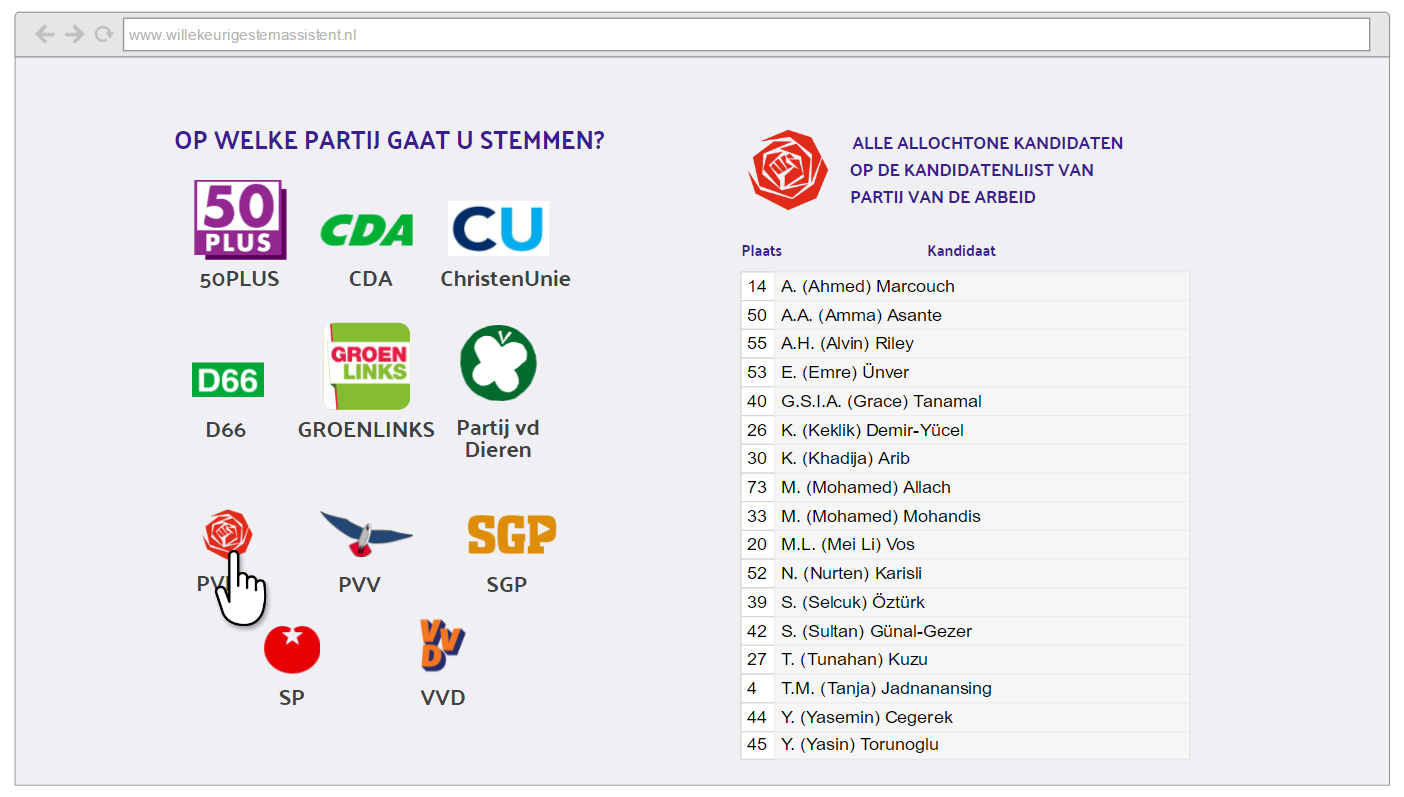
\includegraphics[width=\linewidth]{website_verkiezingen1.png}

			\caption{Website als hulpmiddel die deelnemende leden kan helpen bij het kiezen van een willekeurige kandidaat uit de corresponderende bevolkingsgroep. Dit hulpmiddel kan ook bestaan in de vorm van een mobiele website en een mobiele applicatie.}

\label{fig:verkW}
\end{figure}

In de mock-up wordt strategie 2 uitgevoerd door de bevolkingsgroep allochtonen. De kiezer selecteert de PVDA als de partij waarop zij/hij wilt gaan stemmen en de allochtone kandidaten op de kandidatenlijst van de PVDA worden getoond. De kiezer hoeft nu enkel willekeurig te selecteren uit één van de getoonde allochtone kandidaten. De kiezer kan deze keuze onthouden. Echter is er ook iets te bedenken waardoor de kiezer een reminder zou kunnen ontvangen in de vorm van een sms, een email etc. Het tonen van de foto van de kandidaat is af te raden. Kiezers kunnen op uiterlijk afgaan wanneer zij foto's van de mogelijk te kiezen kandidaten getoond krijgen \citep{banducci2008ballot,lawson2010looking}. 


\paragraph{Hulpmiddel die willekeurige kandidaat selecteert.}
We stellen de tweede IT-toepassing voor die dient als hulpmiddel bij het selecteren van een willekeurige kandidaat conform alle in Hoofdstuk \ref{sec:eva} beschreven strategie\"{e}n. Ook deze toepassing kan al in een vrij simpele vorm bestaan zoals een website en mobiele website maar ook een mobiele applicatie behoort tot de mogelijkheden. Als voorbeeld hebben we echter gekozen voor een mobiele applicatie. In Figuur \ref{fig:verkA} is een mock-up van de mobiele applicatie te zien. Ook hierbij moet genoteerd worden dat de mock-up enkel dient om een beeld te scheten van hoe een hulpmiddel in de vorm van een mobiele website gebruikt zou kunnen worden. Er is hierbij weinig tot geen aandacht besteed aan het ontwerp en de gebruiksvriendelijkheid van de mobiele applicatie.

In de mock-up wordt een strategie uitgevoerd door de bevolkingsgroep vrouwen. Voor het voorbeeld maakt het niet uit welke strategie dit is aangezien alle strategie\"{e}n hierbij van toepassing zijn. In de mock-up in Figuur \ref{fig:verkA} selecteert de kiezer voor GROENLNKS als de partij waarop zij (kan uiteraard ook een hij zijn als mannelijke kiezers willen deelnemen) wilt gaan stemmen en de mobiele applicatie wijst willekeurig een vrouwelijke kandidaat van GROENLINKS aan waarop de kiezer geacht wordt om de stem op uit te brengen. 


\begin{figure}[H]


	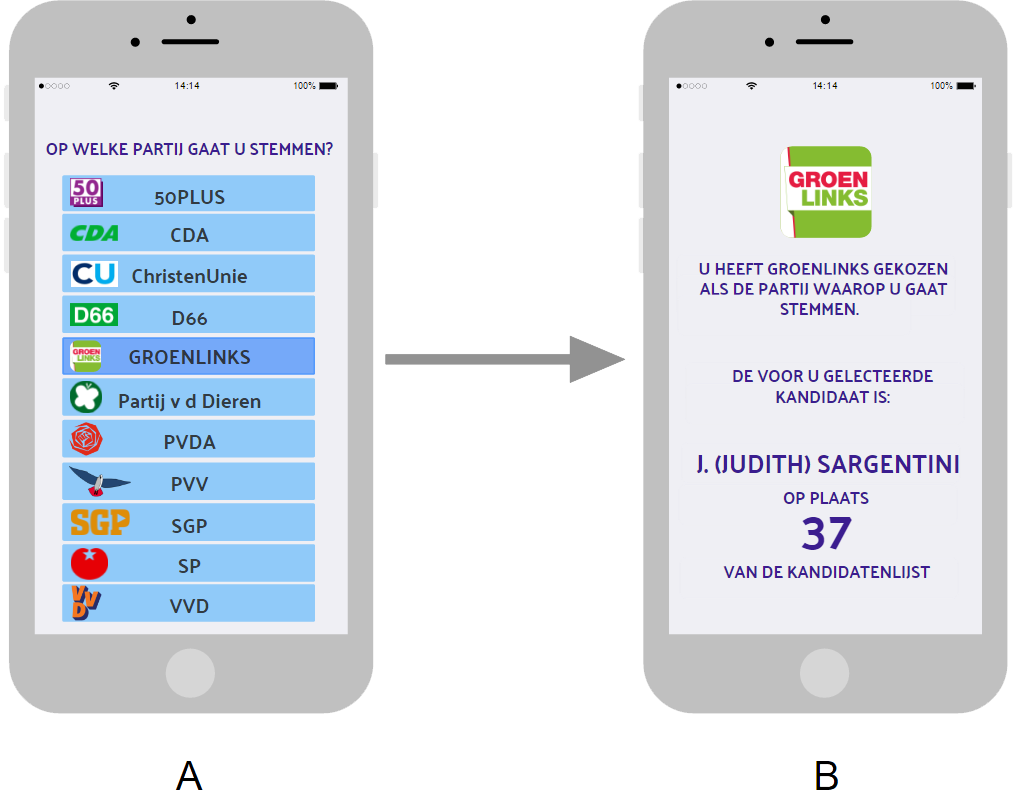
\includegraphics[width=\linewidth]{app_verkiezingen.png}

			\caption{Mobiele applicatie als hulpmiddel die een willekeurige kandidaat uitkiest. Dit hulpmiddel kan ook bestaan in de vorm van een mobiele website en een desktop website.}

\label{fig:verkA}
\end{figure}

In deze sectie hebben we gepoogd een antwoord te verschaffen op hoe een strategie uitgevoerd zou kunnen worden. Waar strategie 2 voor de bevolkingsgroep vrouwen gemakkelijk uitgevoerd kan worden en geen hulpmiddel aan te pas hoeft te komen, is de strategie voor de andere bevolkingsgroepen moeilijker uit te voeren. Een hulpmiddel in de vorm van een IT-toepassing biedt uitkomst. In de volgende sectie gaan we de voor- en nadelen onderzoeken betreffende de keuze voor de wijze waarop een strategie zal worden uitgevoerd. 

\subsection{Voor- en nadelen van keuze voor een uitvoeringswijze strategie.}

\subsection*{Subdeelvraag 3.2: Wat zijn de eventuele voor- en nadelen van de keuze van de wijze waarop een strategie zal worden uitgevoerd?}
In de vorige sectie hebben we een tweetal IT-toepassingen voorgesteld die als hulpmiddel kunnen fungeren bij het uitvoeren van een strategie. Tevens hebben we opgemerkt dat strategie 2 voor de bevolkingsgroep vrouwen vrij gemakkelijk uit te voeren is. In deze sectie zullen we voor- en nadelen gaan onderzoeken van het kiezen voor een bepaalde uitvoeringswijze van een strategie. 

\paragraph{Hulpmiddel en geen hulpmiddel.} 
Vanwege de complexiteit die bij uitvoering van het merendeel van de strategie\"{e}n om de hoek komt kijken hebben we een tweetal hulpmiddelen voorgesteld in de vorm van IT-toepassingen. Echter is het de vraag of er een behoefte zou zijn bij de deelnemende leden van de bevolkingsgroepen op de hulpmiddelen daadwerkelijk te gaan hanteren. \\
\indent Volgens de \textit{Information Richness Theory} \citep{daft1983information} willen mensen onzekerheid zoveel mogelijk pareren bij het uitvoeren van een taak. Hierbij is o.a. een directe terugkoppeling een belangrijk criteria. Voor uitvoering van alle strategie\"{e}n is het dus zaak onzekerheid uit te sluiten wat betreft de mogelijke kandidaten waaruit geselecteerd dient te worden. Enkel bij strategie 2 bij de bevolkingsgroep vrouwen is er een directe terugkoppeling aanwezig om de kandidatenlijst. Bij strategie 2 moeten de kiezers willekeurig een corresponderende kandidaat kiezen en het geslacht van de kandidaat staat op het stemformulier. Zodoende is bij uitvoering van strategie 2 door de bevolkingsgroep vrouwen geen hulpmiddel nodig. Bij de andere strategie\"{e}n bij deze bevolkingsgroep moet er echter uit een top \textit{N} kandidaat worden geselecteerd (zie Hoofdstuk \ref{sec:eva}). Voor de andere strategie\"{e}n geldt dat er zowel een directe terugkoppeling op het stemformulier ontbreekt (strategie 2) alsmede de regels van de strategie te complex kunnen zijn om gemakkelijk toe te passen. \\
\indent Conform de \textit{Theory of Reasoned Action} \citep{fishbein1977belief,ajzen1991theory} en, in het verlengde van deze theorie, de \textit{Technology Acceptance Model} \citep{davis1989perceived,davis1989user, venkatesh2000determinants} zullen kiezers bereidwillig tegenover het gebruik van de technische hulpmiddelen staan wanneer deze hulpmiddelen de uit te voeren taak makkelijker maakt. Zodoende kan worden aangenomen dat in de meeste gevallen een hulpmiddel gewenst is bij het uitvoeren van een strategie. 


\paragraph{Keuze tussen een online of lokale database voor de mobiele applicatie.}
Wanneer een hulpmiddel in de vorm van een mobiele applicatie wordt gehanteerd zijn er enkele factoren wat betreft de data waar rekening mee gehouden dient te worden. Voor het verkrijgen van de data en de informatie te tonen aan de gebruiker van de mobiele applicatie, kan gekozen worden tussen een online database en een lokale database. Echter is ook beiden opties een mogelijkheid.  

De online database zal een \textit{server/client} \citep{Chapt17:online} connectie opzetten waarbij de client de connectie met de server initieert en er data van de server naar de client en andersom gestuurd kan worden. Dit houdt in dat de gebruiker een internet connectie dient te hebben om te zorgen dat, in het geval van strategie 1 en strategie 4, de data ge\"{u}pdatet is a.d.h.v. de laatste peiling. Een dergelijke update zal slechts een kleine hoeveelheid aan data beslaan. Uitgaande van een UTF-8 tekencodering \citep{yergeau2003utf} zou bij de verkiezing van 2012 alle kandidatenlijsten gezamenlijk uitkomen of ongeveer 13 kilobytes. Voor het updaten van enkel de kandidaten die getoond dienen te worden in de mobiele applicatie zal het aantal kilobytes zelfs nog minder zijn (bij strategie 1 ongeveer 4 kilobytes). Er kan ook voor gekozen om de partij-logo's in te laden vanuit de database in plaats van deze al te implementeren in de mobiele applicatie zelf.  Een partij-logo (van 50 bij 50 pixels) zou tussen de 5 en 10 kilobytes zijn wanneer er een PNG-8 bestandstype wordt gebruikt \citep{image39:online,miano1999compressed}. Andere bestandstypes als JPEG en SVG zijn af te raden. Een JPEG bestand is een groter bestand en van mindere kwaliteit dan een PNG-8. Een SVG zou geschikt zijn qua grootte en qua kwaliteit, ware het niet dat een SVG bestand nog niet door alle mobiele besturingssystemen wordt ondersteund \citep{CanIu25:online}. Hoe dan ook, vanwege het feit dat de database slechts een kleine hoeveelheid aan data beslaat (en een update derhalve nog minder) en er verwacht kan worden dat de hoeveelheid data niet zal toenemen zal een kleine database voldoen \citep{silberschatz1997database}. Er kan ook gekozen worden om de keuze van de kiezer bij te houden in de database. Zo kunnen stemmen eventueel effic\"{e}nter gedistribueerd worden over de kandidaten. De kiezer dient in de mobiele applicatie dan wel aan te geven dat de stem is uitgebracht. Om te waarborgen dat een stemkeuze van de kiezer niet meerdere keren in de database wordt opgenomen, en zodoende de database te manipuleren is, wordt via het MAC-adres van het mobiele apparaat van de kiezer (op de verkiezingsdag) bijgehouden of de kiezer de applicatie al heeft gebruikt. Echter lijkt het af te raden om de keuzes van de kiezers op te slaan. Het is immers mogelijk dat een kiezer alsnog voor een andere kandidaat of zelfs een andere partij kiest. In dat geval wordt er incorrecte data naar de database verzonden waarna de kandidaten incorrect gedistribueerd worden. Tevens is het de vraag of het ethisch verantwoord is om op deze manier bij te houden op welke partij een kiezer haar/zijn stem heeft uitgebracht.

Tegenover het gebruik van een online database staat het gebruik van een lokale database ge\"{i}mplementeerd in de mobiele applicatie. Voor een lokale database is geen internet connectie nodig. De database wordt al simpelweg gevuld meegeleverd wanneer de mobiele applicatie wordt ge\"{i}nstalleerd. Een nadeel van een lokale database is echter dat de data in de database eventueel niet actueel is. Peilingen veranderen dagelijks en als een kiezer bijvoorbeeld tien dagen voor de verkiezingen de mobiele applicatie heeft ge\"{i}nstalleerd, is de kans groot dat de data niet meer correspondeert met de laatste peilingen. Zodoende worden op de manier strategie 1 en strategie 4 waarschijnlijk niet optimaal uitgevoerd. Dit kan echter voorkomen worden wanneer de mobiele applicatie na de laatste peilingen aan de vooravond van de verkiezingen wordt ge\"{u}pdatet. Hier is de keizer dan zelf verantwoordelijk voor.

Zowel een online database als een lokale database brengen voor- en nadelen met zich mee. Echter een combinatie van beiden kan uitkomst bieden. Een online database kan een lokale database updaten met de actuele data. Zodra de mobiele applicatie een internet connectie heeft opgezet kan de lokale database opnieuw opgevuld worden aan a.d.h.v. de laatste peiling \citep{silberschatz1997database}. Ook in het geval dat de kiezer ten tijden van het gebruiken van de mobiele applicatie tijdens het uitbrengen van de stem geen internet connectie heeft, kan de laatst opgehaalde data worden getoond aan de kiezer. 





\paragraph{Willekeurige selectie van de kiezer vs. willekeurige toewijzing van een kandidaat aan de kiezer.} Bij het eerste voorgestelde hulpmiddel geeft de kiezer aan welke partij zij/hij wilt gaan stemmen waarna er een lijst wordt getoond met mogelijke kandidaten. Herbij wordt er vanuit gegaan dat de kiezer in staat is een willekeurige keuze te maken. Echter is het zo dat de mens inadequaat is als het gaat om willekeurige keuzes maken en speelt enig vooroordeel vaak een rol \citep{schulz2012analysing,bar1991perception,neuringer1986can}. Om de kiezer hier enigszins bij te ondersteunen zal de lijst altijd in een willekeurige volgorde gepresenteerd worden. De kiezer kan namelijk onbewust een keuze maken op basis van bijvoorbeeld de plaats op de kandidatenlijst wanneer de lijst op volgorde van plaatsnummer wordt gepresenteerd. Om dit zoveel mogelijk te elimineren kan daarom het beste de lijst op een willekeurige volgorde worden gepresenteerd. Echter is de computer d.m.v. het toeassen van een \textit{Pseudorandom Number Generator} (PRNG) veel adequater in het willekeurig kiezen uit bijvoorbeeld een serie getallen of namen dan een mens \citep{lewis1969pseudo,RANDO99:online,matsumoto1998mersenne,rukhin2001statistical}. Zodoende is het de vraag tot in hoeverre het aan de kiezer kan worden overgelaten om een willekeurige keuze te maken uit een lijst met namen zoals het geval zou zijn bij het gebruik van de eerste voorgesteld hulpmiddel. Bij het tweede voorgestelde hulpmiddel wordt  een kandidaat derhalve geselecteerd door de PRNG. Echter is het de vraag of kiezers de keuze voor een kandidaat accepteren wanneer zij deze voorgeschoteld krijgen. Daarom stellen we een ook een derde hulpmiddel voor die gezien kan worden als mengvorm tussen de twee eerder voorgestelde IT-toepassingen. In de mock-up in Figuur \ref{fig:verkC} kan de kiezer zelf een kandidaat selecteren of de groene knop indrukken zodat de computer een kandidaat willekeurig selecteert. Vanwege het feit dat kiezers nog altijd de optie hebben om zelf een kandidaat te selecteren, wordt met deze vorm van de IT-toepassing niet uitgesloten dat kiezers hun stemmen alsnog onevenredig over de kandidaten distribueren. Het is daarom aan te bevelen verder onderzoek te doen naar de meest geschikte toepassingsvorm wanneer een hulpmiddelen in de vorm van een IT-toepassing ontwikkeld gaat worden.  

\begin{figure}[H]


	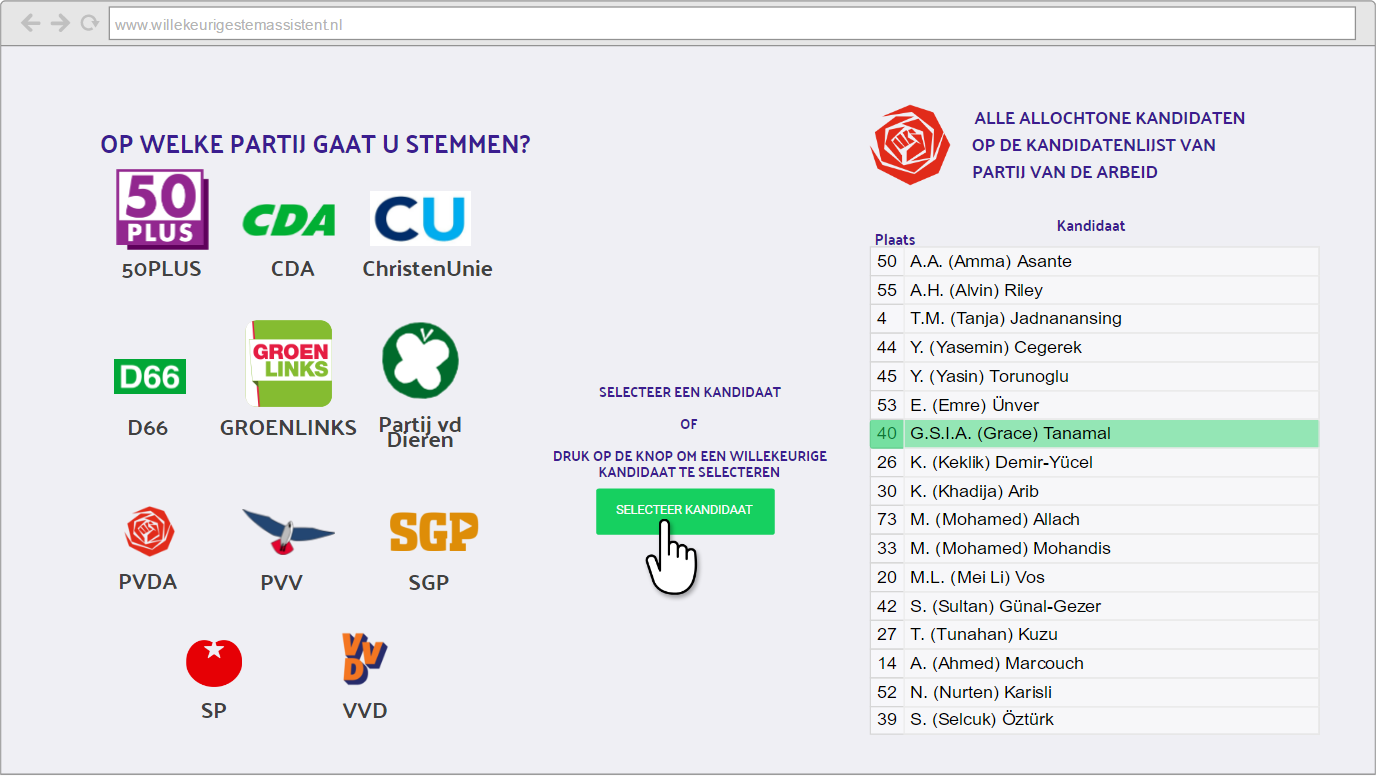
\includegraphics[width=\linewidth]{website_verkiezingen2.png}

			\caption{Derde hulpmiddel, in de vorm van een website, als mengvorm tussen de eerste twee hulpmiddelen. Ook dit hulpmiddel kan ook bestaan in de vorm van een mobiele website en een mobiele applicatie.}

\label{fig:verkC}
\end{figure}







\iffalse
\subsection{Beantwoording Deelvraag}
In deze sectie komen we nog even kort terug te komen op de deelvraag die in dit hoofdstuk is behandeld. De deelvraag luidde: welke strategie is per specifieke bevolkingsgroep aan te bevelen wanneer zij de regel van van voorkeursdrempel in de kieswet uit willen buiten in hun voordeel? Zoals al eerder gez
\fi
\newpage 